\documentclass[12pt]{article}
\usepackage[margin=1in]{geometry}
\usepackage{amsmath,amssymb,amsthm}
\usepackage{graphicx}
\usepackage{tikz}
\usetikzlibrary{arrows.meta,shapes,positioning,calc}
\usepackage{booktabs}
\usepackage{natbib}
\usepackage{hyperref}
\usepackage{xcolor}
\usepackage{enumerate}

\newtheorem{theorem}{Theorem}
\newtheorem{proposition}{Proposition}
\newtheorem{definition}{Definition}

\title{\textbf{The Origin of Codes:\\How Digital Information Emerges from High-Dimensional Chemistry}}

\author{Ian Todd\\
Sydney Medical School\\
University of Sydney\\
Sydney, NSW, Australia\\
\texttt{itod2305@uni.sydney.edu.au}}

\date{}

\begin{document}

\maketitle

\begin{abstract}
The Evolution 2.0 challenge asks how coded information arises from non-living chemistry. We argue the question has the causality backwards. Digital codes are not \textit{built into} chemistry; they \textit{emerge from} the projection of high-dimensional dynamics onto low-dimensional readouts. When diverse chemical species track a common external forcing (the sun, tides), their collective response forms a high-dimensional attractor---many ``ways to track the sun.'' At boundaries (membranes, surfaces), this high-D dynamics projects onto discrete symbols. The transition to life occurs when compartmentalization (lipid bilayers) allows chemistry to swap the external attractor for an endogenously generated one---self-organization replacing sun-organization. We do not need to engineer codes; we need to understand why they inevitably emerge.
\end{abstract}

%==============================================================================
\section{The Challenge Has It Backwards}
%==============================================================================

The Evolution 2.0 prize asks: \textit{How does coded information (encoder $\to$ message $\to$ decoder) arise from purely non-living chemistry?}

This framing assumes:
\begin{itemize}
    \item Digital codes are fundamental and must be \textit{built}
    \item We need to engineer an encoder that produces symbols
    \item The chemistry must somehow ``generate'' discrete states
\end{itemize}

We argue this is backwards. The actual story is:
\begin{itemize}
    \item High-dimensional continuous dynamics are fundamental
    \item ``Digital'' emerges when high-D projects onto low-D at a boundary
    \item Codes are not designed---they are \textit{discovered}
    \item The discreteness is in the \textit{readout}, not the chemistry
\end{itemize}

\begin{quote}
\textbf{Core claim:} Any sufficiently diverse chemistry, tracking a common external forcing, read out at a boundary, automatically produces codes. You don't build codes into chemistry. You find them at the interface.
\end{quote}

%==============================================================================
\section{High-Dimensional Attractors from Common Forcing}
%==============================================================================

\subsection{The Setup}

Consider prebiotic Earth:
\begin{itemize}
    \item \textbf{Diverse chemistry}: Amino acids, sugars, nucleobases, lipids, metal ions, thiols, phosphates---hundreds of species from atmospheric synthesis, meteoric input, hydrothermal vents
    \item \textbf{Common forcing}: The sun (day/night UV, temperature cycling), tides (wet/dry, concentration/dilution), seasons
    \item \textbf{Cross-reactivity}: Everything can react with everything---condensation, complexation, redox, catalysis
\end{itemize}

Each chemical species responds to the forcing in its own way:
\begin{itemize}
    \item Amino acids: photodegradation during day, condensation during dry phases
    \item Sugars: isomerization rates temperature-dependent, formose branching UV-sensitive
    \item Nucleobases: UV absorption drives chemistry, metal complexation shifts with redox
    \item Lipids: phase transitions with temperature, self-assembly concentration-dependent
\end{itemize}

\subsection{The High-Dimensional Attractor}

All these species must track the \textit{same} external rhythm. But each tracks it differently.

\begin{figure}[h]
\centering
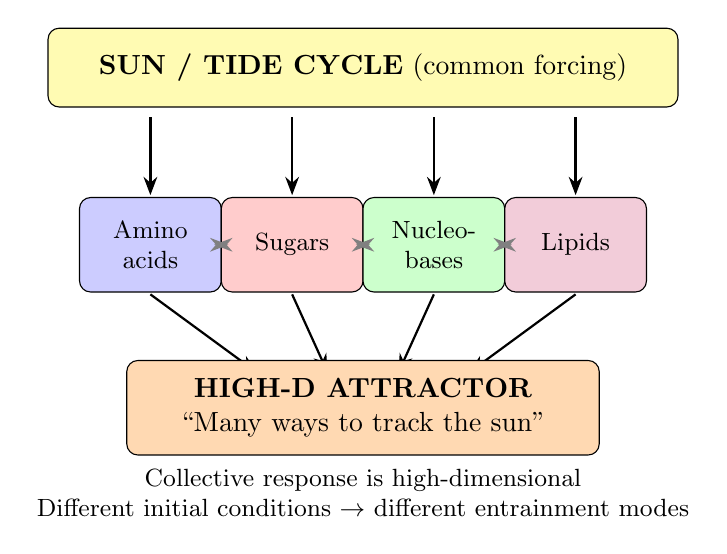
\begin{tikzpicture}[scale=0.9]
    % Sun forcing at top
    \node[draw, rounded corners, fill=yellow!30, minimum width=8cm, minimum height=1cm] at (0,4) {\textbf{SUN / TIDE CYCLE} (common forcing)};

    % Arrows down to different chemistries
    \draw[-{Stealth}, thick] (-3,3.3) -- (-3,2.2);
    \draw[-{Stealth}, thick] (-1,3.3) -- (-1,2.2);
    \draw[-{Stealth}, thick] (1,3.3) -- (1,2.2);
    \draw[-{Stealth}, thick] (3,3.3) -- (3,2.2);

    % Different chemistry boxes
    \node[draw, rounded corners, fill=blue!20, minimum width=1.8cm, minimum height=1.2cm, align=center, font=\small] at (-3,1.5) {Amino\\acids};
    \node[draw, rounded corners, fill=red!20, minimum width=1.8cm, minimum height=1.2cm, align=center, font=\small] at (-1,1.5) {Sugars};
    \node[draw, rounded corners, fill=green!20, minimum width=1.8cm, minimum height=1.2cm, align=center, font=\small] at (1,1.5) {Nucleo-\\bases};
    \node[draw, rounded corners, fill=purple!20, minimum width=1.8cm, minimum height=1.2cm, align=center, font=\small] at (3,1.5) {Lipids};

    % Cross-coupling arrows
    \draw[{Stealth}-{Stealth}, gray, thick] (-2.1,1.5) -- (-1.9,1.5);
    \draw[{Stealth}-{Stealth}, gray, thick] (-0.1,1.5) -- (0.1,1.5);
    \draw[{Stealth}-{Stealth}, gray, thick] (1.9,1.5) -- (2.1,1.5);

    % Arrows down to attractor
    \draw[-{Stealth}, thick] (-3,0.8) -- (-1.5,-0.3);
    \draw[-{Stealth}, thick] (-1,0.8) -- (-0.5,-0.3);
    \draw[-{Stealth}, thick] (1,0.8) -- (0.5,-0.3);
    \draw[-{Stealth}, thick] (3,0.8) -- (1.5,-0.3);

    % High-D attractor
    \node[draw, rounded corners, fill=orange!30, minimum width=6cm, minimum height=1.2cm, align=center] at (0,-0.8) {\textbf{HIGH-D ATTRACTOR}\\``Many ways to track the sun''};

    % Label
    \node[font=\small, align=center] at (0,-2) {Collective response is high-dimensional\\Different initial conditions $\to$ different entrainment modes};
\end{tikzpicture}
\caption{Diverse chemistry tracking a common forcing produces a high-dimensional attractor. Each species responds to the sun/tide cycle in its own way; their collective, coupled response spans many dimensions.}
\label{fig:attractor}
\end{figure}

The collective response is high-dimensional because:
\begin{itemize}
    \item Many species ($n \gg 1$) with partially independent dynamics
    \item Cross-coupling prevents lockstep motion
    \item The ``attractor'' is not a single state but a \textit{manifold} of ways to track the forcing
\end{itemize}

Different initial conditions lead to different positions on this attractor manifold. These are the proto-codes: distinguishable, reproducible, history-dependent states.

%==============================================================================
\section{Digital Emerges at Boundaries}
%==============================================================================

\subsection{The Projection Principle}

The chemistry itself is continuous and high-dimensional. Where do discrete ``symbols'' come from?

\textbf{Answer:} From projection onto low-dimensional readouts at boundaries.

\begin{definition}[Emergent Digitality]
A system exhibits emergent digitality when a high-dimensional continuous dynamics, projected onto a low-dimensional boundary observable, produces distinguishable, reproducible, discrete states---without those states being built into the dynamics.
\end{definition}

\subsection{What Boundaries Do}

Boundaries---membranes, mineral surfaces, phase interfaces---are selective:
\begin{itemize}
    \item \textbf{Membranes}: Only certain molecules permeate; the flux depends on the full chemical state but the \textit{output} is which molecules made it through
    \item \textbf{Surfaces}: Adsorption is selective; different attractor states produce different adsorption patterns
    \item \textbf{Phase interfaces}: Partitioning depends on hydrophobicity, charge, etc.; the oil/water distribution reflects the interior state
\end{itemize}

The boundary acts as a \textbf{coarse-graining operator}. It takes the high-D interior state and projects it onto a few observable dimensions.

\subsection{Why This Creates Discrete Symbols}

When a high-D attractor projects onto a low-D observable, the image is not uniform. It has:
\begin{itemize}
    \item \textbf{Clusters}: Regions of the attractor that map to similar outputs
    \item \textbf{Gaps}: Outputs that no attractor state produces
    \item \textbf{Bistability}: Boundary mechanisms (pH indicators, precipitation thresholds) that snap to discrete states
\end{itemize}

The discreteness is not in the chemistry. It is in the \textit{interface between chemistry and readout}.

\begin{figure}[h]
\centering
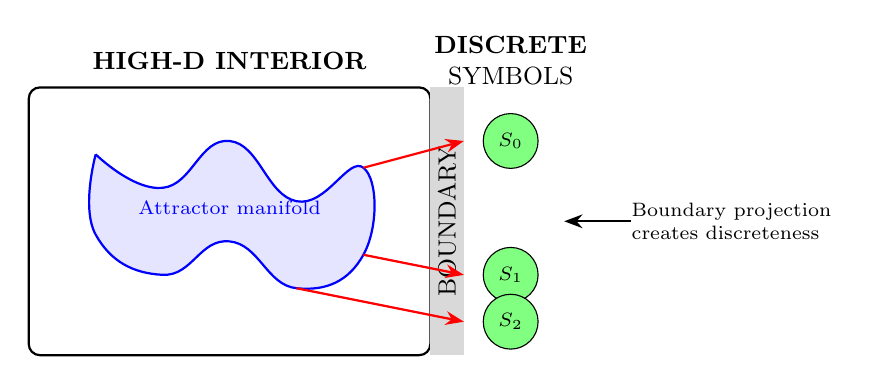
\begin{tikzpicture}[scale=0.85]
    % High-D interior
    \draw[thick, rounded corners] (-3,-2) rectangle (3,2);
    \node[font=\small] at (0,2.4) {\textbf{HIGH-D INTERIOR}};

    % Attractor manifold (wavy shape)
    \draw[thick, blue, fill=blue!10] plot[smooth, tension=0.8] coordinates {(-2,1) (-1,0.5) (0,1.2) (1,0.3) (2,0.8) (2,-0.5) (1,-1) (0,-0.3) (-1,-0.8) (-2,-0.2) (-2,1)};
    \node[font=\scriptsize, blue] at (0,0.2) {Attractor manifold};

    % Boundary (right side)
    \fill[gray!30] (3,-2) rectangle (3.5,2);
    \node[rotate=90, font=\small] at (3.25,0) {BOUNDARY};

    % Projection arrows
    \draw[-{Stealth}, thick, red] (2,0.8) -- (3.5,1.2);
    \draw[-{Stealth}, thick, red] (2,-0.5) -- (3.5,-0.8);
    \draw[-{Stealth}, thick, red] (1,-1) -- (3.5,-1.5);

    % Discrete outputs
    \node[draw, circle, fill=green!50, minimum size=0.5cm, font=\scriptsize] at (4.2,1.2) {$S_0$};
    \node[draw, circle, fill=green!50, minimum size=0.5cm, font=\scriptsize] at (4.2,-0.8) {$S_1$};
    \node[draw, circle, fill=green!50, minimum size=0.5cm, font=\scriptsize] at (4.2,-1.5) {$S_2$};

    % Label
    \node[font=\small, align=center] at (4.2,2.4) {\textbf{DISCRETE}\\SYMBOLS};

    % Annotation
    \draw[{Stealth}-, thick] (5,0) -- (6,0);
    \node[font=\scriptsize, align=left] at (7.5,0) {Boundary projection\\creates discreteness};
\end{tikzpicture}
\caption{Continuous high-D dynamics become discrete symbols at boundaries. The attractor manifold (blue) projects through the boundary onto distinguishable outputs. Discreteness is not built into the chemistry; it emerges from the projection.}
\label{fig:projection}
\end{figure}

%==============================================================================
\section{The Transition to Life}
%==============================================================================

\subsection{Stage 1: External Organization}

Initially, the chemistry tracks an \textit{external} attractor---the sun/tide cycle. The codes that emerge are:
\begin{itemize}
    \item Determined by the external forcing
    \item Reproducible (same forcing $\to$ same attractor region)
    \item History-dependent (initial conditions matter)
\end{itemize}

But the chemistry is not yet ``alive.'' It is organized \textit{by} the sun, not \textit{by itself}.

\subsection{Stage 2: Compartmentalization}

Lipid bilayers form spontaneously in prebiotic conditions. When they encapsulate a subset of the chemistry:
\begin{itemize}
    \item The interior becomes \textit{concentrated}
    \item The boundary becomes \textit{defined} (the membrane)
    \item The interior chemistry can develop its own dynamics, partially decoupled from the external forcing
\end{itemize}

\subsection{Stage 3: Swap the Attractor}

The key transition: inside the compartment, some chemistry becomes \textbf{autocatalytic}---self-amplifying reaction networks that can sustain themselves.

Now the interior dynamics can generate their \textit{own} attractor, independent of the sun.

\begin{quote}
\textbf{The transition to life:} Swap the external attractor (sun-tracking) for an endogenously generated attractor (self-organization). Package it in a lipid bilayer. The ``code'' is now self-maintained.
\end{quote}

\begin{figure}[h]
\centering
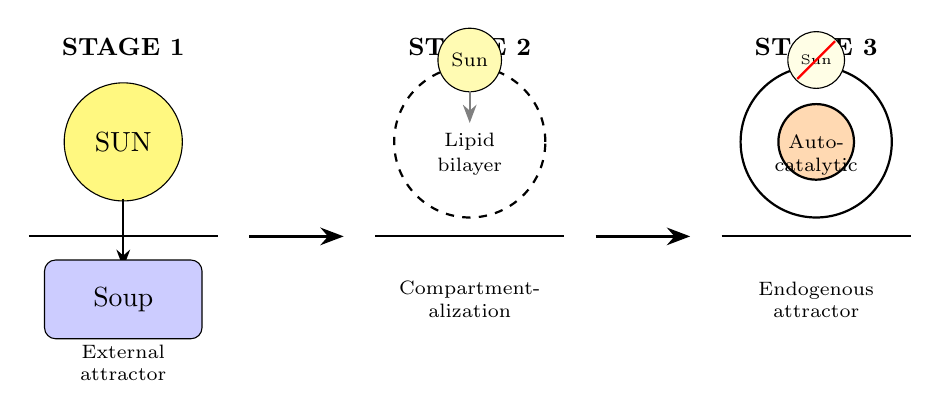
\begin{tikzpicture}[scale=0.8]
    % Stage 1
    \node[font=\small\bfseries] at (-4,3) {STAGE 1};
    \draw[thick] (-5.5,0) -- (-2.5,0);
    \node[draw, circle, fill=yellow!50, minimum size=1.5cm] at (-4,1.5) {SUN};
    \draw[-{Stealth}, thick] (-4,0.6) -- (-4,-0.5);
    \node[draw, rounded corners, fill=blue!20, minimum width=2cm, minimum height=1cm] at (-4,-1) {Soup};
    \node[font=\scriptsize, align=center] at (-4,-2) {External\\attractor};

    % Arrow
    \draw[-{Stealth}, very thick] (-2,0) -- (-0.5,0);

    % Stage 2
    \node[font=\small\bfseries] at (1.5,3) {STAGE 2};
    \draw[thick, dashed] (1.5,1.5) circle (1.2);
    \node[font=\scriptsize] at (1.5,1.5) {Lipid};
    \node[font=\scriptsize] at (1.5,1.1) {bilayer};
    \draw[thick] (0,0) -- (3,0);
    \node[draw, circle, fill=yellow!30, minimum size=0.8cm, font=\scriptsize] at (1.5,2.8) {Sun};
    \draw[-{Stealth}, thick, gray] (1.5,2.3) -- (1.5,1.8);
    \node[font=\scriptsize, align=center] at (1.5,-1) {Compartment-\\alization};

    % Arrow
    \draw[-{Stealth}, very thick] (3.5,0) -- (5,0);

    % Stage 3
    \node[font=\small\bfseries] at (7,3) {STAGE 3};
    \draw[thick] (7,1.5) circle (1.2);
    \draw[thick, fill=orange!30] (7,1.5) circle (0.6);
    \node[font=\scriptsize] at (7,1.5) {Auto-};
    \node[font=\scriptsize] at (7,1.1) {catalytic};
    \draw[thick] (5.5,0) -- (8.5,0);
    \node[font=\scriptsize, align=center] at (7,-1) {Endogenous\\attractor};

    % Crossed out sun
    \node[draw, circle, fill=yellow!10, minimum size=0.6cm, font=\tiny] at (7,2.8) {Sun};
    \draw[thick, red] (6.7,2.5) -- (7.3,3.1);

\end{tikzpicture}
\caption{The transition to life. Stage 1: Chemistry tracks external attractor (sun). Stage 2: Compartmentalization in lipid bilayer. Stage 3: Internal autocatalytic network generates its own attractor; external forcing becomes optional. Life = chemistry that organizes itself.}
\label{fig:transition}
\end{figure}

%==============================================================================
\section{What ``Digital'' Actually Means}
%==============================================================================

The Evolution 2.0 challenge demands a ``digital'' system. But what does digital mean in chemistry?

\subsection{The Wrong Answer}

\textbf{Wrong:} The chemistry has discrete states built in.

This is the assumption behind looking for ``chemical bits''---molecules that are either ON or OFF, reactions that are either HAPPENED or DIDN'T.

The problem: chemistry is fundamentally continuous. Concentrations vary smoothly. Reaction rates are continuous functions of temperature, pH, etc.

\subsection{The Right Answer}

\textbf{Right:} The readout has discrete states, because the boundary mechanism is bistable/multistable.

``Digital'' is not a property of the interior dynamics. It is a property of the \textit{interface}.

Examples of physically discrete readouts:
\begin{itemize}
    \item \textbf{pH indicators}: Sharp color transitions at threshold pH
    \item \textbf{Precipitation}: Either precipitate forms or it doesn't
    \item \textbf{Phase transitions}: Lipid gel vs fluid phase
    \item \textbf{Membrane permeation}: Above threshold concentration, molecules cross; below, they don't
\end{itemize}

In each case, the interior chemistry is continuous; the readout snaps to discrete values because of the \textit{physics of the boundary}, not because of ``digital chemistry.''

\subsection{Implications for Evolution 2.0}

The challenge asks: ``Show chemistry generating digital information.''

Our answer: Chemistry doesn't generate digital information. Chemistry is continuous and high-dimensional. Digital information \textit{emerges at boundaries} when high-D dynamics project onto bistable readouts.

If you want to see codes:
\begin{enumerate}
    \item Take diverse chemistry (many species)
    \item Apply common forcing (sun/tide cycle)
    \item Read out at a boundary (membrane, surface)
    \item The codes are there---you discover them, you don't design them
\end{enumerate}

%==============================================================================
\section{The Experimental Realization}
%==============================================================================

\subsection{System Design}

Based on the above framework, a compliant experimental system is:

\textbf{Substrate} (the ``soup''):
\begin{itemize}
    \item Amino acids: Gly, Ala, Asp, Glu, Ser, Val, Leu, Ile, Pro, Phe (10 species)
    \item Sugars: Ribose, glucose, glyceraldehyde, formaldehyde, glycolaldehyde (5 species)
    \item Nucleobases: Adenine, guanine, cytosine, uracil (4 species)
    \item Metal ions: Fe$^{2+}$, Mg$^{2+}$, Zn$^{2+}$, Ca$^{2+}$ (4 species)
    \item Phosphate, thiols (cysteine), fatty acids (2--3 species)
    \item Total: $\sim$25--30 primary species, plus reaction products
\end{itemize}

\textbf{Forcing} (the ``sun''):
\begin{itemize}
    \item UV cycling: 12h on / 12h off (or accelerated: 1h cycles)
    \item Temperature cycling: 20°C $\to$ 60°C $\to$ 20°C
    \item Wet/dry cycling: Partial evaporation then rehydration
\end{itemize}

\textbf{Boundary} (the ``readout''):
\begin{itemize}
    \item Option A: Mineral surface (montmorillonite clay)---measure adsorption pattern
    \item Option B: Lipid vesicles---measure permeation/internal composition
    \item Option C: Phase interface---measure partitioning into oil phase
\end{itemize}

\textbf{Readout mechanism} (bistable for digitality):
\begin{itemize}
    \item pH indicator dyes in readout compartment (discrete color states)
    \item Precipitation assay (Ca$^{2+}$ + oxalate: precipitate or not)
    \item Turbidity threshold (lipid aggregation: clear or cloudy)
\end{itemize}

\subsection{Protocol}

\begin{enumerate}
    \item Prepare substrate mixture in buffer with mineral surface or vesicles
    \item Define input conditions: 64 combinations of (forcing phase, initial pH, metal ratio, concentration)
    \item Run system for 10--100 forcing cycles
    \item Sample boundary readout at end of each cycle
    \item Record discrete state (which indicator state, which precipitation pattern)
    \item Repeat 10 trials per input condition
\end{enumerate}

\subsection{Expected Outcomes}

\begin{itemize}
    \item Different input conditions $\to$ different boundary patterns
    \item Patterns cluster into discrete states (symbols) without imposed thresholds
    \item Reproducibility $>$70\% (same input $\to$ same symbol)
    \item $\geq$32 distinct symbols observed
\end{itemize}

The codes are \textit{discovered} by clustering the observed outputs, not \textit{designed} by choosing thresholds.

%==============================================================================
\section{Mapping to Evolution 2.0 Requirements}
%==============================================================================

\begin{center}
\begin{tabular}{lll}
\toprule
\textbf{Requirement} & \textbf{Our System} & \textbf{Note} \\
\midrule
Encoder & High-D soup + forcing & Attractor selection \\
Message & Boundary flux/composition & Chemical intermediates \\
Decoder & Bistable indicator & Physical discretization \\
Symbol & Discrete readout state & Emergent, not imposed \\
Character & Sequence over cycles & $M^n$ states \\
$\geq$32 states & $4^3 = 64$ & Satisfies requirement \\
Digital & Boundary bistability & Physics, not binning \\
No pre-programming & Codes discovered & Tables populated empirically \\
No biological material & Synthetic reagents & All commercial \\
\bottomrule
\end{tabular}
\end{center}

%==============================================================================
\section{Why the Challenge is Backwards}
%==============================================================================

The Evolution 2.0 challenge implicitly assumes:
\begin{enumerate}
    \item Codes are designed/engineered
    \item Digital is fundamental
    \item We need to find ``the right chemistry''
\end{enumerate}

We have argued:
\begin{enumerate}
    \item Codes emerge inevitably from high-D dynamics + boundaries
    \item Digital is a projection artifact, not a fundamental property
    \item Any sufficiently diverse chemistry works---there is no ``right'' chemistry
\end{enumerate}

The transition to life was not the \textit{invention} of codes. It was:
\begin{enumerate}
    \item High-D chemistry tracking external forcing (codes emerge at boundaries)
    \item Compartmentalization (lipid bilayer defines the boundary)
    \item Swapping external attractor for endogenous one (self-organization)
    \item Learning to read and replicate the boundary states (evolution)
\end{enumerate}

Life didn't create information. It \textit{exapted} the codes that physics was already producing at the interface between high-dimensional chemistry and low-dimensional readouts.

%==============================================================================
\section{Conclusion}
%==============================================================================

We have presented a framework for understanding how coded information emerges from non-living chemistry:

\begin{enumerate}
    \item \textbf{High-dimensional dynamics}: Diverse chemistry tracking common forcing creates a high-D attractor (``many ways to track the sun'')
    \item \textbf{Boundary projection}: Discrete symbols emerge when high-D projects onto low-D at boundaries (membranes, surfaces)
    \item \textbf{Emergent digitality}: The discreteness is in the readout physics (bistability), not the chemistry
    \item \textbf{Transition to life}: Compartmentalization + autocatalysis allows chemistry to swap external for endogenous attractors
\end{enumerate}

The Evolution 2.0 challenge asks how to build codes into chemistry. We have shown that codes are not built---they emerge. The question is not ``how do we engineer an encoder?'' but ``why do boundaries inevitably produce symbols?''

The answer: because projection from high-D to low-D, through a bistable interface, is a discretizing operation. Codes are not invented. They are discovered at the interface between complex dynamics and simple readouts.

This is not a limitation to be engineered around. It is the mechanism by which life arose.

\vspace{1em}
\noindent\rule{\textwidth}{0.4pt}
\vspace{0.5em}
\noindent\textbf{Submitted to}: HeroX Evolution 2.0 Prize

\end{document}
